% !TeX root = construct.tex

\selectlanguage{hebrew}
\chapter[\R{ איך לחלק זווית לשלושה חלקים )אם אתם מוכנים לרמות( }]%
{איך לחלק זווית לשלושה חלקים\\)אם אתם מוכנים לרמות(}
\label{c.trisect-an-angle}

%%%%%%%%%%%%%%%%%%%%%%%%%%%%%%%%%%%%%%%%%%%%%%%%%%%%%%%%%%%%%

ידוע שלא ניתן לחלק זווית שרירותית לשלושה  חלקים שווים בעזרת מחוגה וסרגל. הסיבה היא שחלוקת זווית לשלושה דורשת בנייה של שורש שלישי, אבל עם מחוגה וסרגל ניתן לבנות רק אורכים המתקבלים מארבעת פעולות החשבון וכן שורש ריבועי.

המתמטיקאים היוונים גילו שבאמצעות כלים אחרים ניתן לחלק זווית לשלושה. סעיף~%
\L{\ref{s.neusis}}
מציג בנייה של ארכימדס עם כלי פשוט הנקרא ביוונית ניאוסיס
\L{(neusis)}.
סעיף~%
\L{\ref{s.q}}
מביא בנייה מסובכת יותר של היפיאס באמצעות
\qd{}
\L{(quadratrix)}.
כהטבה מיוחדת, נראה בסעיף~%
\L{\ref{s.square}}
איך ניתן לרבע מעגל באמצעות 
\qd{}.


מקורות:

\selectlanguage{english}
\noindent\url{https://en.wikipedia.org/wiki/Angle_trisection}\\
\url{https://en.wikipedia.org/wiki/Quadratrix_of_Hippias}\\
\url{https://en.wikipedia.org/wiki/Neusis_construction}
\selectlanguage{hebrew}

\vspace{-2ex}

%%%%%%%%%%%%%%%%%%%%%%%%%%%%%%%%%%%%%%%%%%%%%%%%%%%%%%%%%%%%%

\section{חלוקת זווית לשלושה באמצעות ניאוסיס}\label{s.neusis}

השימוש במילה "סרגל" מטעה, כי הכוונה היא למקל ישר ללא כל סימן, שהפעולה היחידה שניתן לעשות איתו היא למתוח קו ישר בין שתי נקודות. לסרגל המוכר יש סימנים המאפשרים למדוד אורכים. כדי לחלק זווית לשלושה חלקים, נשתמש ב-%
\textbf{ניאוסיס}
שהוא מקל עם שני סימנים בלבד. נניח שהמרחק בין שני הסימנים הוא
$1$:
\begin{center}
\selectlanguage{english}
\begin{tikzpicture}[scale=3.5]
\draw (-1,1.05) rectangle +(3.2,.1);
\draw[thick] (1.89,1.05) -- +(0,.1);
\draw[thick] (.73,1.05) -- +(0,.1);
\draw[<->] (.73,1.25) -- node[fill=white] {$1$} (1.89,1.25);
\end{tikzpicture}
\end{center}
תהי 
$\alpha$
זווית שרירותית
$\angle ABE$
בתוך מעגל שמרכזו
$B$
עם רדיוס
$1$.
ניתן לבנות את המעגל על ידי קביעת המרחק בין רגלי החוגה למרחק בין סימני הניאוסיס. בנו קרן כהמשכו של 
$EB$
מחוץ למעגל. הניחו את הניאוסיס על הנקודה
$A$
והזיזו אותו עד שהוא חותך את הקרן בנקודה 
$D$
ואת המעגל בנקודה
$C$.
כוונו את הניאוסיס כך שהאורך של
$CD$
יהיה
$1$.
ציירו את הקו
$AD$:


\begin{center}
\selectlanguage{english}
\begin{tikzpicture}[scale=2.5]
\coordinate (origin) at (0,0) node[below] {$B$} ;
\draw[name path=circle] (origin) circle [radius=1];
\draw (origin) node[above left,xshift=-4pt] {$\alpha$} -- (120:1) coordinate (a) node[below,xshift=-2pt] {$A$} ;
\draw (-1,0) -- (2.2,0);
\path[name path=ad] (a) -- (0,0 -| 2,0) coordinate (d) node[below] {$D$} ;
\path[name intersections={of=circle and ad,by={c,a1}}];
\fill (origin) circle [radius=.5pt];
\fill (a) circle [radius=.5pt];
\fill (c) circle [radius=.5pt] node [below,xshift=-4pt] {$C$};
\fill (d) circle [radius=.5pt];
\fill (-1,0) circle [radius=.5pt] node [left] {$E$};
\begin{scope}[rotate=-19,yshift=-11.25pt]
\draw (-1,1.05) rectangle +(3.2,.1);
\draw[thick] (1.89,1.05) -- +(0,.1);
\draw[thick] (.76,1.05) -- +(0,.1);
\draw[<->] (.73,1.25) -- node[fill=white] {$1$} (1.89,1.25);
\end{scope}
\end{tikzpicture}
\end{center}

\np

ציירו את הקו 
$BC$
וסמנו את הזוויות וקטעי הקו בתרשים:
\begin{center}
\selectlanguage{english}
\begin{tikzpicture}[scale=2.5]
\coordinate (origin) at (0,0) node[below] {$B$} ;
\draw[name path=circle] (origin) circle [radius=1];
\draw (origin) node[above left,xshift=-4pt] {$\alpha$} node[above,xshift=4pt,yshift=2pt] {$\delta$} node[above right,xshift=44pt,yshift=-2pt] {$\beta$} -- node[fill=white] {$1$} (120:1) coordinate (a) node[above left] {$A$} ;
\draw (-1,0) -- (2.2,0);
\draw[name path=ad] (a) node[below right,xshift=8pt,yshift=-6pt] {$\gamma$} -- (0,0 -| 2,0) coordinate (d) node[left,xshift=-50pt,yshift=7pt] {$\beta$} node[above right] {$D$} ;
\path[name intersections={of=circle and ad,by={c,a1}}];
\draw (origin) -- node[fill=white] {$1$}(c) node[above right] {$C$} node[left,xshift=-12pt] {$\gamma$} node[below,xshift=-2pt,yshift=-2pt] {$\epsilon$};
\fill (origin) circle [radius=.5pt];
\fill (a) circle [radius=.5pt];
\fill (d) circle [radius=.5pt];
\fill (c) circle [radius=.5pt];
\fill (-1,0) circle [radius=.5pt];
\path (c) -- node[fill=white] {$1$} (d);
\end{tikzpicture}
\end{center}

$BA=BC$
כי שניהם רדיוסים ו-%
$CB=CD$
לפי הבניה באמצעות הניאוסיס. לכן 
$\triangle ABC$, $\triangle BCD$
שווי שוקיים. החישוב שלהלן משתמש בעובדות שסכום הזוויות של משולש ושל זוויות משלימות הוא
$180^\circ$:

\vspace{-3ex}

\erh{2pt}
\begin{equationarray*}{rcl}
\epsilon &=& 180^\circ - 2\beta\\
\gamma &=& 180^\circ - \epsilon = 2\beta\\
\delta &=& 180^\circ - 2\gamma = 180^\circ - 4\beta\\
\alpha &=& 180^\circ - \delta - \beta = 4\beta -\beta =3\beta\,.
\end{equationarray*}
\vspace{-2ex}
הזווית
$\beta$
היא שליש מהזווית
$\alpha$.
%%%%%%%%%%%%%%%%%%%%%%%%%%%%%%%%%%%%%%%%%%%%%%%%%%%%%%%%%%%%%


\section{חלוקת זווית לשלושה באמצעות
\qd{}%
}\label{s.q}

התרשים שלהלן מראה
\textbf{מחוגת \qd{}}
המורכב משני סרגלים )ללא סימנים( המחוברים במפרק המאלץ אותם לנוע ביחד. סרגל אחד נע במקביל לציר ה-%
$x$
מ-%
$DC$
עד
$AB$.
הסרגל השני מחובר לנקודה
$A$
ומסתובב ממצב אנכי לאורך 
$AD$
עד שהוא במצב אופקי לאורך 
$AB$. 
העקומה המצוירת על ידי המפרק המחבר את שני הסרגלים נקראת
\textbf{עקומת ה%
\qd{}%
}
או פשוט
\textbf{\qd{}}.
\begin{center}
\selectlanguage{english}
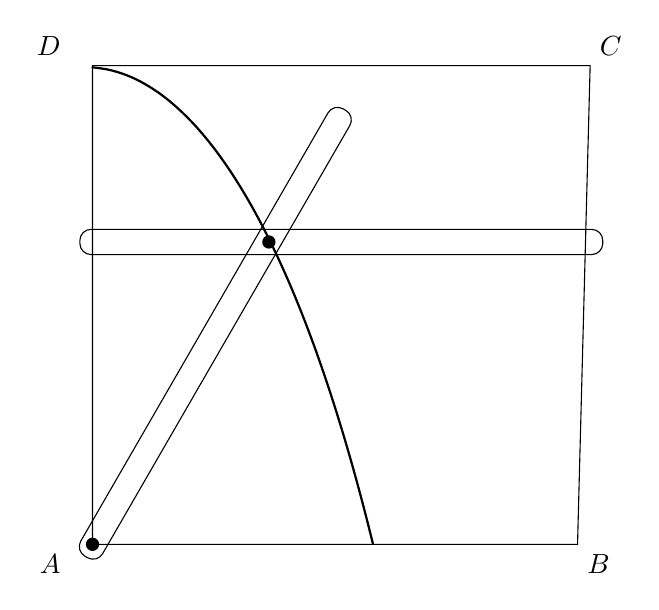
\begin{tikzpicture}[scale=.8,domain=.03:1.555,samples=100]
\draw (.1,.2) node[below left,xshift=-8pt] {$A$} -- (7.8,.2) node[below right] {$B$} -- (8,7.8) node[above right] {$C$} -- (.1,7.8) node[above left,xshift=-8pt] {$D$} -- cycle;
%\draw (.1,7.8) -- (.1,.2) -- (8,.1) -- (8,7.8);
\draw[rounded corners,rotate=60] (0,-.2) rectangle (8.2,.2);
\draw[rounded corners] (-.1,4.8) rectangle (8.2,5.2);
\fill (2.9,5) circle [radius=3pt];
\fill (.1,.2) circle [radius=3pt];
\draw[thick] plot (4.6*.637*\x,{12.2*.637*\x*cot(\x r)});
\end{tikzpicture}
\end{center}

\np

כאשר מזיזים את הסרגל האופקי במהירות אחידה, החיבור מאלץ את הסרגל השני להסתובב במהירות זוותית קבועה. למעשה זו ההגדרה של ה%
\qd{}.
כאשר קואורדינטת ה-%
$y$
של הסרגל האופקי יורד מ-%
$1$
ל-%
$0$,
הזווית של הסרגל השני יחסית לציר ה-%
$x$
יורד מ-%
$90^\circ$
ל-%
$0^\circ$.
התרשים שלהלן מראה איך אפשר לחלוק זווית שרירותית 
$\alpha$
לשלושה חקלים שווים באמצעות
\qd{}:

\vspace{-2ex}

\begin{center}
\selectlanguage{english}
\begin{tikzpicture}[scale=.8,domain=.03:1.562,samples=100]
\draw (.1,7.8) coordinate (start) node[above left] {$D$} node[below right,xshift=32pt] {$\theta$} -- (.1,.2) node[below left] {$A$} -- (8,.1) node[below right] {$B$} -- (8,7.8) node[above right] {$C$} -- cycle;
\draw[name path=curve,thick] plot (4.6*.637*\x,{12.2*.637*\x*cot(\x r)});
\path[name path=twenty] (start) -- +(-35:9);
\path[name path=sixty] (start) -- +(-50:9);
\path[name path=xaxis] (.1,.2) -- (8,.1);
\path[name intersections={of=twenty and curve,by={x1,tri}}];
\draw (start) -- (tri);
\fill (tri) circle [radius=2pt] node[right] {$P_2$};
\path[name intersections={of=sixty and curve,by={x2,angle}}];
\fill (angle) circle [radius=2pt] node[right] {$P_1$};
\draw (start) -- (angle);
\path[name intersections={of=xaxis and curve,by=x}];
\fill (x) circle [radius=2pt];
%\path (.1,.2) -- node[below] {$2/\pi$} (x);
\draw[dashed] (tri) -- (tri -| .1,.2) coordinate (t3);
\fill (t3) circle [radius=2pt] node[left] {$F$};
\draw[dashed] (angle) -- (angle -| .1,.2) coordinate (t);
\fill (t) circle [radius=2pt] node[left] {$E$};
\draw[<->] (-1.2,7.8) -- node[fill=white] {$t/3$} (-1.2,7.8 |- t3);
\draw[<->] (-.6,7.8) -- node[fill=white] {$t$} (-.6,7.8 |- t);
\draw[<->] (-.6,7.8 |- t) -- node[fill=white] {$1-t$} (-.6,.2);
\draw (3.5,7.8) arc[start angle=0,delta angle=-49,radius=3.5];
\draw (1,7.8) arc[start angle=0,delta angle=-32,radius=1];
\node at (3.3,6) {$\alpha$}; 
\end{tikzpicture}
\end{center}

\vspace{-3ex}

הנקודה
$P_1$
היא החיתוך בין הקו המגדיר את הזווית 
$\alpha$
לבין ה%
\qd{}.
קואורדינטת ה-%
$y$
שלה היא
$1-t$,
כאשר 
$t$
הוא המרחק שהסרגל האופקי נע ממקומו ההתחלתי
$DC$.
חלק את
$DE$
לשלושה חלקים כדי לקבל את הנקודה
$F$.
)קל לחלק
\textbf{קטע הקו}
לחלקים שווים על ידי שימוש במשפט תאלס(. הנקודה
$P_2$
היא נקודת החיתוך בין הקו מ-%
$F$
המקביל ל-%
$DC$
לבין ה%
\qd{}.
לפי העיקרון של מהירויות שוות:

\vspace{-4ex}

\erh{12pt}
\begin{equationarray*}{rcl}
\frac{\theta}{\alpha} &=& \frac{t/3}{t}\\
\theta &=& \alpha/3\,.
\end{equationarray*}

%\vspace{-8ex}
\newpage

%%%%%%%%%%%%%%%%%%%%%%%%%%%%%%%%%%%%%%%%%%%%%%%%%%%%%%%%%%%%%

\section{ריבוע מעגל באמצעות
\qd{}%
}\label{s.square}


\begin{center}
\selectlanguage{english}
\begin{tikzpicture}[scale=.8,domain=.01:1.57,samples=100]
\draw (0,0) node[below left] {$A$} node [above right,xshift=10pt] {$\theta$} -- (8,0) node[below right] {$B$} -- (8,8) node[above right] {$C$} -- (0,8) node[above left] {$D$} -- cycle;
\draw[name path=horiz] (0,5) -- (8,5);
\draw[name path=slant] (0,0) -- (61:8);
\path[name intersections={of=horiz and slant,by=joint}];
\draw[dashed] (joint) -- node[right] {$y$} (joint |- 0,0) coordinate (f);
\path (0,0) -- node[below] {$x$} (0,0 -| joint) node[below] {$F$};
\path (0,5) node[left] {$E$} -- node[left] {$t$} (0,8);
\path (0,0) -- node[left] {$1-t$} (0,5);
\fill (joint) circle [radius=2pt] node[above right,xshift=4pt] {$P$};
\fill (f) circle [radius=2pt];
\fill (0,5) circle [radius=2pt];
\fill (4.28,0) circle [radius=2pt] node[below] {$G$};
\draw[name path=curve,thick] plot (4.3*.637*\x,{12.5*.637*\x*cot(\x r)});
\end{tikzpicture}
\end{center}


נניח שהסרגל האופקי נע מרחק 
$t$
לאורך ציר ה-%
$y$
עד לנקודה
$E$,
ושהסרגל המסתובב מגדיר זווית 
$\theta$
עם ציר ה-%
$x$.
הנקודה 
$P$
היא החיתוך בין
\qd{}
לבין הסרגל האופקי, והנקודה
$F$
היא היטל של 
$P$
על ציר ה-%
$x$.
מהן הקואורדינטות של הנקודה 
$P$
על ה%
\qd{}?
ברור ש:
\[
y=PF=EA=1-t\,.
\]
על העקומה,
$\theta$
יורד באותו קצב ש-%
$t$
עולה:
\erh{12pt}
\begin{equationarray*}{rcl}
\frac{1-t}{1} &=& \frac{\theta}{\pi/2}\\
\theta &=&\frac{\pi}{2}(1-t)\,.
\end{equationarray*}
נבדוק אם זה הגיוני: כאשר
$t=0$
אז
$\theta=\pi/2$,
וכאשר
$t=1$
אז
$\theta=0$.

את קואורדינטת ה-%
$x$
של
$P$
נקבל בטריגונומטריה:
\[
\tan \theta = \frac{y}{x}\,.
\]
ומכאן:

\[
x = \frac{y}{\tan\theta}=y\cot\theta=y\cot \frac{\pi}{2}(1-t)=y\cot \frac{\pi}{2}y\,.
\]

בדרך כלל המשוואה של עקומה היא מהצורה
$y=f(x)$,
אבל אפשר גם להשתמש במשוואה מהצורה
$x=f(y)$.
נחשב את קוארדינטת ה-%
$x$
של הנקודה 
$G$,
החיתוך של ה%
\qd{}
עם ציר ה-%
$x$.
לא ניתן להציב
$y=0$
כי
$\cot 0$
לא מוגדר, אבל ייתכן שיהיה לנו מזל אם נחשב את הגבול של
$x$
כאשר 
$y$
שואף ל-%
$0$:

\[
x = y\cot \frac{\pi}{2}y = \frac{2}{\pi}\cdot \frac{\pi}{2}y\cot \frac{\pi}{2}y\,.
\]

למען הנוחיות, נחליף משתנה
$z=\disfrac{\pi}{2}y$,
ואז נחשב את הגבול:

\[
\lim_{z\rightarrow 0} z\cot z = \lim_{z\rightarrow 0} \frac{z\cos z}{\sin z} = \lim_{z\rightarrow 0} \frac{\cos z}{\disfrac{\sin z}{z}} = \frac{\cos 0}{1} = 1\,,
\]

השתמשנו בעובדה הידועה ש-%
$\lim_{z\rightarrow 0} \disfrac{\sin z}{z}=1$.

כאשר
$y\rightarrow 0$:

\[
x \rightarrow \frac{2}{\pi}\cdot \lim_{y\rightarrow 0}\frac{\pi}{2}y\cot \frac{\pi}{2}y = \frac{2}{\pi}\cdot 1 = \frac{2}{\pi}\,.
\]

על ידי שימוש ב%
\qd{}
בנינו קטע קו
$AG$
שאורכו
$x=\disfrac{2}{\pi}$.
עם סרגל רגיל ומחוגה, קל לבנות קו באורך
$\sqrt{\pi}=\sqrt{\disfrac{2}{x}}$,
ואז לבנות ריבוע ששטחו
$\pi$.

\selectlanguage{english}
